\documentclass[a4paper,12pt]{article}
% Package to make citations superscrit with brackets
\usepackage[super,square]{natbib}
% Package to change margin size
\usepackage{anysize}
\usepackage{amsmath}
\marginsize{2cm}{2cm}{1cm}{2cm}
% Package to make headers
\usepackage{fancyhdr}
\renewcommand{\headrulewidth}{0pt}
% Package for highligths
\usepackage{soul}
% Colors for the references links
\usepackage[dvipsnames]{xcolor}
% Package to link references
\usepackage{hyperref}
\hypersetup{
    colorlinks=true,
    linkcolor=black,
    citecolor=CadetBlue,
    filecolor=CadetBlue,      
    urlcolor=CadetBlue,
}
% Package for lorem ipsum
\usepackage{lipsum}
% Package for multicolumn
\usepackage{multicol}
% Package for removing paragraph identations
\usepackage{parskip}
\setlength\columnsep{18pt}
% Sets bastract
\renewenvironment{abstract}
 {\par\noindent\textbf{\abstractname}\ \ignorespaces \\}
 {\par\noindent\medskip}

\usepackage{amssymb}
\usepackage{tabularx} 
\usepackage{graphicx}
\usepackage{longtable}
\usepackage{float}

 
\begin{document}
% Makes header
\pagestyle{fancy}
\thispagestyle{empty}
\fancyhead[R]{\textit{IE522: Statistical Methods in Finance}}
\fancyhead[L]{}
% Makes footnotes with an asterisk
\renewcommand*{\thefootnote}{\fnsymbol{footnote}}
\begin{center}
\Large{\textbf{University of Illinois Urbana-Champaign}}
\vspace{0.4cm}
\normalsize
\textit{}
\medskip
\normalsize
\end{center}
{\color{gray}\hrule}
\vspace{0.4cm}

    \vspace*{2cm} % Vertical spacing at the top
    
    \begin{center}
        
    {\LARGE \textbf{Statistical Methods in Finance}} \\[0.5cm] % Replace 'Course Name' with the actual name
    {\large Course Code: IE: 522} \\[0.5cm] % Replace 'XYZ 123' with the actual course code
    
    \vspace{2cm} % More vertical space
    
    {\Large \textbf{Enhanced Monte Carlo Methods for Option Pricing}} \\[1cm] % Replace with your assignment title
    
    \textbf{Submitted by:}

\begin{table}[h!]
\centering
\begin{tabular}{|l|}
\hline
\textbf{Name} \\ \hline
Aakash Bansal \\ \hline
Michael Bhang \\ \hline
Saurabh Jamadagni \\ \hline
Yifan Meng \\ \hline
\end{tabular}
\caption{ Authors}
\label{tab:uin_names}
\end{table}

    
    \vspace{1.5cm}
    
    \textbf{Submitted to:} \\[0.2cm]
    {\large Dr. Liming Feng} \\ % Replace with your instructor's name
    
    \vfill % Pushes remaining text to bottom
    
    {\large Date: December 17, 2024} % Automatically uses today's date

\end{center}


{\color{gray}\hrule}
\medskip
\newpage
{\color{gray}\hrule}
\begin{center}
\section{Abstract}
\bigskip
\end{center}
{\color{gray}\hrule}
\vspace{0.5cm}
This study offers critical insights into the effectiveness and limitations of numerical methods for option pricing, contributing to their practical utility in financial modeling and risk management. We focus on using numerical methods to price three types of financial options: European vanilla put options, Asian call options, and American vanilla put options, using the Black Scholes Merton model. Each type of option comes with its own challenges, from handling price movement in Asian options to managing early exercise in an American option.

For European and Asian options, we use Monte Carlo simulations to estimate the option price, enhanced through techniques such as antithetic variates, control variates, and moment matching to improve efficiency and reduce variance. For American options, the Longstaff-Schwartz method is employed to account for the early exercise option, and we compare its performance with the Binomial Black Scholes with Richardson Extrapolation (BBSR) method.

The study explores how key parameters—sample size (\(N\)), time steps (\(M\)), and regression order (\(K_{\text{reg}}\))—affect the pricing accuracy, convergence, and computational efficiency of these numerical approaches. For European options, results show the theoretical convergence rates (\(1 / N\)) with a significant reduction in standard error and narrowing of confidence intervals as \(N\) increases. Asian options introduce path dependency, addressed through variance reduction and moment matching techniques, leading to improved precision in option estimates. For American options, the Longstaff-Schwartz method shows sensitivity to \(N\), \(M\), and \(K_{\text{reg}}\), but convergence to the BBSR benchmark highlights its effectiveness.

Results from extensive numerical experiments reveal practical tradeoffs between accuracy and computational cost across all methods. The BBSR method emerges as a highly stable and accurate benchmark, particularly for American options, while the Longstaff-Schwartz method provides greater flexibility for complex derivatives. Recommendations are provided to balance computational efficiency and accuracy, along with future directions for integrating variance reduction techniques and parallelization which can improve the performance in real-world applications.


\newpage
\tableofcontents
\newpage
    {\color{gray}\hrule}
\begin{center}
\section{Introduction}
% \textbf{You can add small descriptions of what the current sections describe}
\bigskip
\end{center}
{\color{gray}\hrule}

\begin{multicols}{2}
Option pricing plays a vital role in finance, helping to value derivatives and manage risks effectively. Here, we focus on pricing three different options: European, Asian, and American using the Black Scholes Merton framework and Monte Carlo simulations. European options are simpler and based on a fixed payoff at maturity, Asian options depend on the average price of the underlying asset over time, and American options add complexity by allowing early exercise.
\subsection{Background on the Monte Carlo methods for option pricing}
Monte Carlo simulations are used for option pricing because they can handle complicated payoff scenarios and model a variety of predictons. We explore how Monte Carlo methods can be used to price these options, analyze their accuracy as sample sizes increase, and evaluate computational efficiency. We also implement techniques like antithetic variates, control variates, and Richardson extrapolation to improve results and performance. For American options, we compare the Longstaff-Schwartz\cite{VAOSSLSA} method with other approaches to understand their accuracy and effectiveness. Our report aims to provide practical insights into the strengths and limitations of these methods in option pricing.
\subsection{Black Scholes Merton for option pricing}
The Black-Scholes-Merton (BSM) model is one of the most widely used methods for pricing options. Introduced in the 1970s\cite{POCL}, it provides a formula to determine the fair price of an option. The model assumes that the price of an underlying asset follows a Brownian motion, with continuously compounded returns, constant volatility, and no arbitrage.

For European options, the BSM model\cite{TBSM} calculates the price by estimating its expected payoff and discounting it at the risk free interest rate. For a call option, the price is given by the formula\cite{522SLIDES}:
\[C = e^{-rT} \mathbb{E} [(S_T-K)^+]\]
\[
C = S_0 e^{-qT}\phi(d_+) - K e^{-rT} N(d_-)\]
\[d_{\pm} = \frac{log(\frac{S0}{k}) + (r - q \pm \frac{1}{2}\tilde{\sigma}^2)T}{\tilde{\sigma}\sqrt{T}}\]
\[\sigma = \tilde{\sigma}\sqrt{T}\]
where:

\begin{itemize}
    \item \( S_0 \): The current price of the underlying asset
    \item \( K \): The strike price of the option
    \item \( T \): The time to maturity (in years)
    \item \( r \): The risk-free interest rate
    \item \( \sigma \): The volatility of the asset
    \item \( \phi(d) \): The cumulative probability of \( d \) under a standard normal distribution.
\end{itemize}
\subsection{Objectives}
Our goal is to explore and apply advanced numerical techniques for option pricing under the Black-Scholes-Merton framework. This includes evaluating the performance of Monte Carlo simulation methods for different types of options and implementing enhancements to improve computational efficiency.
\begin{itemize}
    \item To apply Monte Carlo simulations for pricing European, Asian, and American options under Black Scholes Merton model.
    \item To analyze the convergence and accuracy of Monte Carlo methods as the sample size increases.
    \item To evaluate computational efficiency and performance improvement through advanced techniques such as antithetic variates, control variates, and moment matching.
    \item To compare the Longstaff-Schwartz method for pricing American options with the Binomial Black-Scholes with Richardson Extrapolation (BBSR) approach for accuracy.
    \item To understand the impact of key parameters, such as the number of paths, time steps, and regressors, on the pricing accuracy and computational time.
\end{itemize}


\end{multicols}
\newpage


{\color{gray}\hrule}
\begin{center}
\section{European Vanilla Put Option Pricing}
% \textbf{You can add small descriptions of what the current sections describe}
\bigskip
\end{center}
{\color{gray}\hrule}
\begin{multicols}{2}

\subsection{Problem Statement}
Pricing a European Vanilla Option is a key concept in financial engineering. Here, we are pricing a put option, which gives the buyer the right and not the obligation to sell an asset at a fixed price, called the strike price (\(K\)), on a future date (\(T\)). 

The payoff at maturity depends on how the asset price (\(S_T\)) compares to \(K\) and is calculated as:
\[\text{Payoff} = \max(0, K - S_T)
\]
If the asset price falls below the strike price, the option has value; otherwise, it expires worthless. 

The theoretical price of this option is calculated using the Black-Scholes-Merton model, which considers the expected value of the payoff, adjusted for the time value of money:
$$
    p = e^{-rT} \mathbb{E}[\max(0, K - S_T)]
$$
Here:
\begin{itemize}
    \item \(r\): the risk-free interest rate, which accounts for continuous compounding.
    \item \(K\): the strike price of the option.
    \item \(S_T\): the asset price at maturity.
\end{itemize}

In this project, our goal is to estimate the price of the option using Monte Carlo simulations, which use random sampling to approximate the expected value. We'll also explore how increasing the number of simulations (\(N\)) improves accuracy. 

The results will include:
\begin{itemize}
    \item Estimated option price.
    \item Error margins and confidence intervals (CI).
    \item Computation time.
    \item Difference from the exact Black-Scholes price.
\end{itemize}

\subsection{Methodology}

For N simulations, we create a new instance of the \texttt{Option} class. Each instance initializes values according to the Problem setup discussed further. The stock price is simulated using random numbers generated using the normal distribution. Based on these prices at t=T, the payoff is calculated, discounted and returned for that particular price path. We then take the arithmetic average across all such N paths which gives the final value for the option.

The sample mean $(\mathbb{E}[P])$ and the mean of the square of price $(\mathbb{E}[{P^2})$ which gives the standard error,

$$
    se(Payoff) = \sqrt{\frac{\mathbb{E}[{P^2}] - (\mathbb{E}[P])^2}{N - 1}}
$$

We can construct the 100(1-$\alpha$)\% confidence interval using the Central limit theorem and the above standard error for the estimate.

\subsubsection{Problem Setup}

We aim to price an European Put option using Monte Carlo simulations under the following setup:

\begin{itemize}
    \item Spot price $(S_o) = \$100$
    \item Strike price $K = \$100 $
    \item Time to Maturity $(T)$ = 0.5 year
    \item Risk-free Rate $(r) = 4\%$
    \item Dividend yield $(q) = 2\%$
    \item Volatility $(\sigma) = 20\%$
\end{itemize}

The convergence of the Monte Carlo method is evaluated by varying the number of simulated paths (N) and analyzing the results. We vary N by a factor of 4. This is in line with the theoretical convergence of $1/\sqrt{n}$ for Monte Carlo. By varying by a factor of 4, we aim to observe a reduction in standard error by \textbf{half}.

\subsubsection{Variance Reduction Technique: Antithetic Approach\cite{POUDEL}}

The Antithetic variate approach uses a synthetic asset which is perfectly negatively correlated with the original asset. The synthetic asset is called the antithetic variate. Consider the assets,

$dS_{1,t} = rS_{1,t}dt + \sigma S_{1,t}dZ_t$

$dS_{1,t} = rS_{1,t}dt - \sigma S_{1,t}dZ_t$

The r, $\sigma$, time to maturity are all the same and the starting price is also the same. Thus, the analytical value of the option for both these paths will be the same. If the two options were combined, we would observe $var(0.5(S_1+S_2)) < var(S_1)$ and $var(0.5(S_1+S_2)) < var(S_2)$\cite{POUDEL}. This is because the assets are negatively correlated. Any movement results in  negative co-movement and thus the resulting payoff observes very less movement.

We then have the following payoffs for our put option,
$$
    P_{T} = (K - S(0) exp(\sqrt{T}+\sigma \sqrt{T}(Z))^+
$$
$$
    P_{T}^* = (K - S(0)exp(\sqrt{T}+\sigma \sqrt{T}(-Z))^+
$$
where, $Z \thicksim \mathcal{N}(0,1)$. In our simulation, we can then take the mean of these two payoffs and assign it as our final payoff for the put option.

%Richardson Extrapolation is used to enhance the accuracy of Monte Carlo simulation results by reducing the bias associated with discretization. The approach involves:
%\begin{itemize}
%   \item Running simulations at two different levels of granularity.
%    \item Combining results to cancel out leading-order error terms.
%\end{itemize}
%Imagine you're trying to measure something, but your tools aren’t perfect—they give you slightly different results depending on how precise you try to be. Richardson Extrapolation helps you combine those results to cancel out the main errors and get a better answer.
\subsection{Results}
The following table(Table 1) summarizes the results of the Monte Carlo simulation, showing the option price, estimated standard error (SE), 95\% confidence interval, absolute pricing error, and computation time for different sample sizes (\(N\)).

\subsubsection{Convergence Analysis}
\textbf{Option Price and Absolute Error:}  
European Option price estimate for the selected parameters with an accuracy upto a cent is \textbf{\$5.07}. 

As the sample size increased, the estimated option price steadily converged toward the true value. At \(N = 256,000\), the absolute pricing error was minimal at just 0.002222, demonstrating a highly accurate estimate. Beyond this sample size, further increases provided only marginal improvements in accuracy, indicating diminishing returns.


\textbf{Estimated Standard Error (SE):}  
The standard error decreased with larger sample sizes, reflecting greater precision in the estimates. For \(N = 4,096,000\), the SE was as low as 0.00354899, highlighting the reliability of the simulation at higher sample sizes. 

We can clearly observe that the standard error is halved every time the number of simulations is increased by 4, which is in line with the $\frac{1}{\sqrt{n}}$ convergence of Monte Carlo.

\textbf{Confidence Intervals:}  
The 95\% confidence intervals narrowed significantly as the sample size grew, offering greater certainty in the estimated price. For \(N = 4,096,000\), the interval was \([5.06534, 5.07925]\), indicating a high degree of confidence in the results.

\end{multicols}
\begin{table}[h!]
\centering
\caption{Summary of Results}
\begin{tabular}{|p{1.8cm}|p{1.8cm}|p{2cm}|p{4cm}|p{2cm}|p{2cm}|}
\hline
\textbf{Sample Size (\(N\))} & \textbf{Option Price} & \textbf{Estimated SE} & \textbf{95\% C.I.} & \textbf{Absolute Pricing Error} & \textbf{Compute Time (s)} \\ \hline
1,000      & 5.62406  & 0.24316   & [5.14747, 6.10064] & 0.549421  & 0.001396 \\ \hline
4,000      & 5.32484  & 0.115344  & [5.09877, 5.55091] & 0.250203  & 0.004458 \\ \hline
16,000     & 5.13141  & 0.0568855 & [5.01992, 5.2429]  & 0.056773  & 0.017990 \\ \hline
64,000     & 5.0646   & 0.0283004 & [5.00913, 5.12007] & 0.010036  & 0.074846 \\ \hline
256,000    & 5.07241  & 0.0142032 & [5.04458, 5.10025] & 0.002222  & 0.228177 \\ \hline
1,024,000  & 5.08877  & 0.00711048 & [5.07483, 5.10271] & 0.014134  & 0.875244 \\ \hline
4,096,000  & 5.07229  & 0.00354899 & [5.06534, 5.07925] & 0.002343  & 3.53752  \\ \hline
20,000,000  & 5.07678  & 0.00177545 & [5.0733, 5.08026] & 0.002147  & 17.457s  \\ \hline
\end{tabular}
\end{table}
\begin{figure}
    \centering
    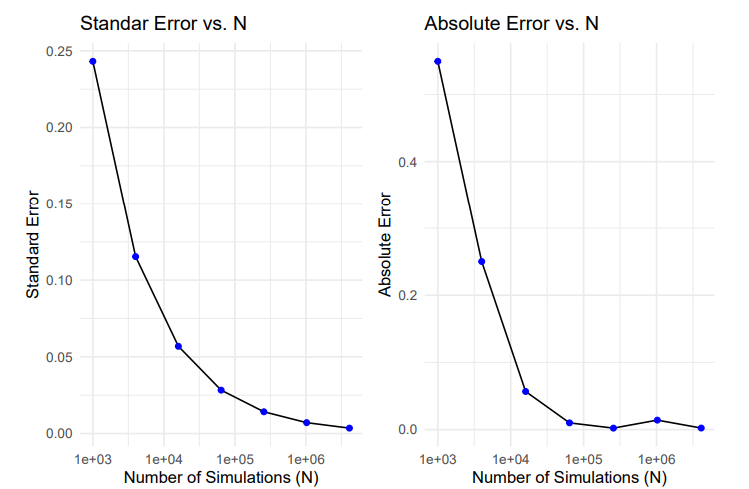
\includegraphics[width=0.8\linewidth]{1.png}
    \caption{Error - Simulations}
    \label{fig:enter-label}
\end{figure}
\begin{multicols}{2}
\subsubsection{Computational Performance}
\textbf{Computation Time:}  
The computation time increased proportionally with the sample size. For \(N = 1,000\), the simulation completed in just 0.001396 seconds, whereas for \(N = 4,096,000\), it required 3.53752 seconds, reflecting the tradeoff between precision and computational demand.

\textbf{Efficiency-Accuracy Tradeoff:}  
While larger sample sizes improved accuracy and precision, they also demanded significantly more computational resources. For practical purposes, \(N = 256,000\) strikes a good balance between accuracy and efficiency, delivering results with minimal error and reasonable computation time.

\subsubsection{Antithetic Approach}
The antithetic variates approach is used in Monte Carlo simulations to make option pricing more accurate and efficient. Instead of using random samples, it creates pairs of related samples that are negatively correlated. For example, if a random movement in the underlying asset price is generated, an opposite movement is also created by using the opposite signs for the random numbers. By averaging the results of these paired paths, the approach reduces random fluctuations and provides a more stable estimate of the option price. 
\end{multicols}
\begin{table}[h!]
\centering
\caption{Antithetic Method Results}
\vspace{4pt}
\begin{tabular}{|p{1.8cm}|p{1.8cm}|p{2cm}|p{4cm}|p{2cm}|p{2cm}|}
\hline
\textbf{Sample Size (\(N\))} & \textbf{Option Price} & \textbf{Estimated SE} & \textbf{95\% Confidence Interval} & \textbf{Absolute Pricing Error} & \textbf{Compute Time (s)} \\ \hline
256,000    & 5.07394  & 0.00710851 & [5.06001, 5.08787] & 0.000698  & 0.196551 \\ \hline
20,000,000  & 5.07427  & 0.000888735 & [5.07253, 5.07602] & 0.000362  & 16.9786  \\ \hline
\end{tabular}
\end{table}
\begin{figure}
    \centering
    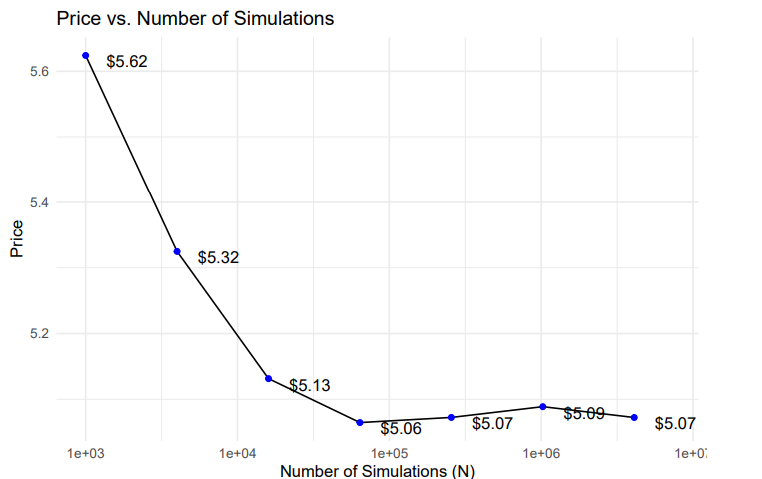
\includegraphics[width=0.8\linewidth]{2.png}
    \caption{Price - Simulations}
    \label{fig:enter-label}
\end{figure}
\begin{multicols}{2}
\textbf{Improved Accuracy:}  
For the optimal sample size of \(N = 256,000\):
\begin{itemize}
    \item \textbf{Standard Monte Carlo:} Option price = 5.07241 with an absolute pricing error of 0.002222.
    \item \textbf{Antithetic Method:} Option price = 5.07394 with an absolute pricing error of 0.000698.
\end{itemize}
The antithetic approach significantly reduces the absolute error while maintaining the same number of samples.

\textbf{Lower Standard Error:}  
The Estimated Standard Error (SE) is consistently lower using the antithetic method:
\begin{itemize}
    \item For \(N = 256,000\), SE = 0.00710851 in the antithetic method versus 0.0142032 in the standard method.
    \item For \(N = 20,000,000\), SE reduces further to 0.000887758 in the antithetic method.
\end{itemize}
This demonstrates that the antithetic variates technique achieves higher precision with reduced variance.

\textbf{Narrower Confidence Intervals:}  
The 95\% confidence intervals are narrower with the antithetic method, indicating greater certainty in the estimates.

\textbf{Comparable or Better Computational Efficiency:}  
While the computation time increases slightly with larger \(N\), the antithetic method achieves a more accurate and precise result. For example:
\begin{itemize}
    \item For \(N = 20,000,000\), the antithetic method required 16.9786 seconds, whereas the standard Monte Carlo took 17.457 seconds.
\end{itemize}

In summary, the antithetic variates approach not only improves accuracy and precision but also demonstrates computational efficiency, making it a superior choice for pricing options using Monte Carlo methods.
\subsection{Discussion}

The results of the Monte Carlo simulations for pricing the European vanilla put option demonstrate the impact of sample size and variance reduction techniques, particularly the antithetic variates approach, on accuracy, precision, and computational efficiency.
\subsubsection{Comparison of Methods}

The comparison between the standard Monte Carlo method and the antithetic variates approach clearly highlights the advantages of the latter. The absolute pricing error using the antithetic method was reduced compared to the standard method. The antithetic method consistently produced a smaller standard error and the 95\% confidence intervals were significantly narrower indicating greater certainty in the option price estimate.
\subsubsection{Convergence Behavior}
The results validate the theoretical convergence rate of \(1/\sqrt{N}\) for Monte Carlo simulations. As the sample size \(N\) increased, the option price approached the true value, and the standard error decreased proportionally. However, the effect diminished for very large \(N\) where increases in sample size gave us marginal improvements in accuracy and required significantly more compute time.  Additionally, in comparison to the standard Monte Carlo method, the antithetic method achieved more accurate results in slightly less time (e.g., 16.9786s for \(N = 20,000,000\)).
\end{multicols}
\begin{figure}
    \centering
    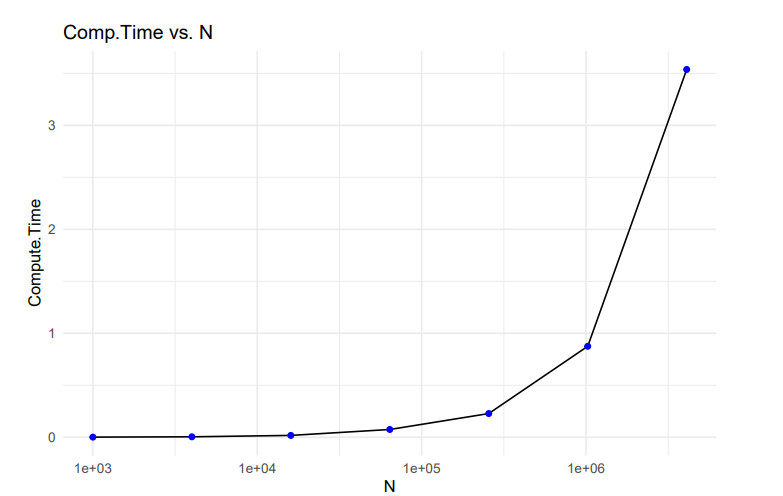
\includegraphics[width=0.8\linewidth]{3.png}
    \caption{Computation Time - Simulations}
    \label{fig:enter-label}
\end{figure}
\begin{figure}
    \centering
    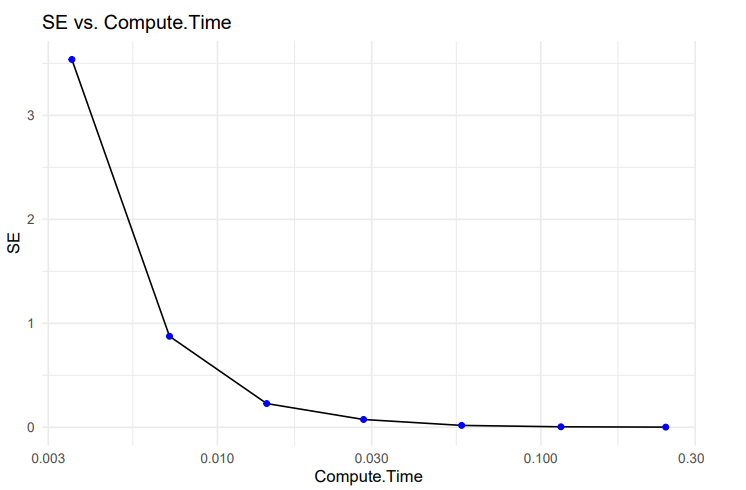
\includegraphics[width=0.8\linewidth]{4.png}
    \caption{Computation Time - Standard Error}
    \label{fig:enter-label}
\end{figure}
\begin{multicols}{2}
This highlights the efficiency-accuracy tradeoff: the antithetic variates approach delivers better results with minimal additional computational cost, making it particularly valuable for time-sensitive applications.
\subsubsection*{Practical Implications of Variance Reduction}
The antithetic method proves to be a powerful variance reduction technique for Monte Carlo simulations. By generating negatively correlated movements and averaging their payoffs, the method reduces random fluctuations, improves accuracy, and decreases standard error without requiring a significant increase in the sample size.

In real-world applications, such as financial risk management or high frequency trading, where computational resources are limited, the antithetic approach can provide faster, more reliable option pricing results.
\subsubsection*{Limitations and Future Work}
While the antithetic method significantly improves accuracy and precision, it may not be sufficient for options with more complex payoffs, such as path-dependent options or American options. Future work can explore combining antithetic variates with other variance reduction techniques, such as control variates or stratified sampling, to achieve even better results. Additionally, leveraging parallel computing could help reduce computational time for very large \(N\).
\subsubsection{Key Insights}
\begin{itemize}
    \item The antithetic variates method reduces variance and improves the accuracy of Monte Carlo simulations without an increase in the computation time.
    \item For practical purposes, a sample size of \(N = 256,000\) strikes an effective balance between accuracy and efficiency.
    \item The method’s ability to produce narrower confidence intervals and lower standard errors makes it a valuable enhancement for option pricing models.
\end{itemize}

\end{multicols}

\newpage
{\color{gray}\hrule}
\begin{center}
\section{Asian Call Option Pricing}
% \textbf{You can add small descriptions of what the current sections describe}
\bigskip
\end{center}
{\color{gray}\hrule}
\begin{multicols}{2}

\subsection{Problem Statement}
An Asian call option is unique because its payoff depends on the average price of the underlying asset over a certain period, rather than just the price at maturity. \cite{PAOMCC} They are popular due to their reduced sensitivity to market manipulation and lower volatility compared to European options.

In the Black-Scholes-Merton model, this average price, \(\overline{S}_T\), is calculated as:
\[
\overline{S}_T = \frac{1}{m} \sum_{i=1}^{m} S_{t_i}\]
where:
\begin{itemize}
    \item \(t_i = i \Delta t\), 
    \item \(\Delta t = \frac{T}{m}\), 
\end{itemize}
with \(T\) being the time to maturity and \(m\) the number of time intervals.

At maturity, the payoff of the Asian call option is determined using the formula:
\[
\text{Payoff} = \max(0, \overline{S}_T - K)
\]
where \(K\) is the strike price. 

The theoretical price of the Asian call option\cite{PAOMCC} is given by:
\[
c = e^{-rT } \mathbb{E}[\max(0, \overline{S}_T - K)]
\]
where:
\begin{itemize}
    \item \(r\): the risk-free interest rate (continuously compounded),
    \item \(\mathbb{E}\): the expected value operator.
\end{itemize}

The objective of this project is to estimate the price of the Asian call option\cite{PAOBOMCC} using Monte Carlo simulation. We will evaluate how the accuracy of the method improves as the sample size \(N\) increases. The results will include:
\begin{itemize}
    \item The estimated option price,
    \item Confidence intervals,
    \item Computational time.
\end{itemize}

\subsection{Methodology}

\subsubsection{Problem Setup}

We aim to price an Asian Call option using Monte Carlo simulations under the following setup:

\begin{itemize}
    \item Spot price $(S_o) = \$100$
    \item Strike price $K = \$100 $
    \item Time to Maturity $(T)$ = 1 year
    \item Risk-free Rate $(r) = 10\%$
    \item Dividend yield $(q) = 0\%$
    \item Volatility $(\sigma) = 20\%$
    \item Number of steps $(m) = 50$
\end{itemize}

Similar to the European put option pricing problem, the convergence of the Monte Carlo method is evaluated by varying the number of simulated paths (N) and analyzing the results. We vary N by a factor of 4. This is in line with the theoretical convergence of $1/\sqrt{n}$ for Monte Carlo. By varying by a factor of 4, we aim to observe a reduction in standard error by \textbf{half}.

\subsubsection{Challenges and Considerations}

\begin{itemize}
    \item Computational Cost: The accuracy of Monte Carlo simulations improves with N, but this comes at the cost of higher computational time.
    \item Variance Reduction Techniques: Methods such as antithetic variates, control variates, or importance sampling can accelerate convergence by reducing variance. We revisit the control variate method in \ref{subsec: 3.2.3}
    \item Discretization Error: The approximation of the continuous time model with discrete time steps introduces discretization error, which can be mitigated by increasing m.
\end{itemize}

\subsubsection{Control Variate technique\cite{AOPMCCV}}
\label{subsec: 3.2.3}

The method of variance reduction using control variates works based on the underlying concept that in order to estimate a quantity from data, information about another estimator can be used to adjust the original estimator. The other estimator used as the source of information is considered the control.

For this problem, we use the geometric Asian call price as our control. We take advantage of the fact that we can calculate the analytical value of the geometric Asian call using the Black-Scholes formula. This is because the geometric average shares a key property with stock price which is the lognormal distribution.\cite{PAOBOMCC}

We define the aritmetic mean $\bar{S_A}$ and the geometric mean $\bar{S_G}$ of stock prices as,
$$
    \bar{S_A} = \frac{1}{m} \sum_{j=1}^m S(t_j)\cite{PAOBOMCC}
$$
$$
    \bar{S_G} = \frac{1}{m} \sum_{j=1}^m log(S(t_j))\cite{PAOBOMCC}
$$
Payoff of the geometric Asian call is given similar to other call options, $(\bar{S_G} - K, 0)^+$

\textbf{Black-Scholes formula for the Analytical Geometric Asian Call price}\cite{PAOBOMCC}

$G_{bs} = e^{-r^*T} \left[S(0)e^{r^*T}\cdot\phi(D1)-K\phi(D2)\right]$\cite{TBSM}

$D1 = \frac{log(S(0)/K) + (r^* + \frac{1}{2}\sigma^{*2})T}{\sigma^*\sqrt{T}}$\cite{TBSM}

$D2 = D1 - \sigma^*\sqrt{T}$\cite{TBSM}

$\sigma^* = \sigma^2 \cdot \frac{(m+1)(2m+1)}{6m^2}$\cite{TBSM}

where, $\phi(\cdot)$ is the cumulative distribution function of the standard normal distribution, $\mathcal{N}(0,1)$.

Our goal is to obtain information for our Monte Carlo estimator using the geometric prices. 

Let $C_A, C_G$ be the value of the arithmetic and geometric Asian call respectively. Let $C_{CV}$ represent the adjusted estimator. We have,
$$
    C_{CV} = C_A + \hat{a}(C_G - G_{bs})
$$
We need to find the value of $\hat{a}$ which gives us reduced variance for the same sample size. Note, irrespective of the value of $\hat{a}$, $C_CV$ is an unbiased estimator of arithmetic Asian option price as $\mathbf{E}[C_G] = G_{bs}$.

The correlation of $C_A$ and $C_G$ is observed to be very close to 1. This implies, variance can be highly reduced by assuming $\hat{a} = -1$. Therefore,
$$
    C_{CV} = C_A + (G_{bs} - C_G)
$$
% \subsubsection{Moment Matching approach}
% \text{}
\subsubsection{Moment Matching Approach}

The moment matching approach is used to reduce variance in the Monte Carlo simulations to improve the efficiency of option pricing. The idea is to adjust the simulated sample paths so that their moments (mean and variance) match the theoretical moments calculated for the underlying asset's price distribution using the Black-Scholes-Merton model. This makes sure that the simulated samples better represent the behavior of the asset price, leading to a reduction in the variability.

\textbf{Key Concept:}  
In the Black-Scholes-Merton framework, the underlying asset price (\(S_t\)) follows a lognormal distribution. The key moments of this distribution at time \(T\) are:
\begin{itemize}
    \item \textbf{Mean:} \(\mathbb{E}[S_T] = S_0 e^{(r-q)T}\),
    \item \textbf{Variance:} \(\text{Var}[S_T] = S_0^2 e^{2(r-q)T}(e^{\sigma^2 T} - 1)\).
\end{itemize}

The moment matching approach modifies the simulated asset prices so that:
\begin{itemize}
    \item The mean of the simulated prices matches \(\mathbb{E}[S_T]\),
    \item The variance of the simulated prices matches \(\text{Var}[S_T]\).
\end{itemize}

We are interested in fitting the log-normal distribution to match the moments. A log-normal distribution is a random variable whose logarithm follows a normal distribution and is characterized by its skewed shape with a fat right tail, which allows it to capture outliers better than the normal distribution. Because of such property, it is frequently used in finance to model stock prices or asset returns.

Given the first and second moments $\mathbb{E}[X]=m_1$ and $\mathbb{E}[X^2]=m_2$ of the observations, $\mu$ and $\sigma$ can be estimated\cite{chan2015moments}:

\begin{itemize}
    \item $\mu=\ln(\frac{m_1^2}{\sqrt{m2}})$
    \item $\sigma=\sqrt{\ln(\frac{m_2}{m_1^2})}$
\end{itemize}

Using the estimated {$\mu$} and {$\sigma$}, the price of Asian call ($C$) and put ($P$) can be obtained\cite{chan2015moments}:

$C=e^{\mu-rT+\frac{1}{2}\sigma^2}\Phi(\frac{\mu-\ln K + \sigma^2}{\sigma})-Ke^{-rT}\Phi(\frac{\mu-\ln K}{\sigma})$
$P=Ke^{-rT}\Phi(\frac{\ln K-\mu}{\sigma})-e^{\mu-rT+\frac{1}{2}\sigma^2}\Phi(\frac{\ln K -\mu - \sigma^2}{\sigma})$

\textbf{Application to Asian Options:}  
For Asian options, the average asset price (\(\overline{S}_T\)) is a function of multiple time steps. So, to apply moment matching:
\begin{enumerate}
    \item Simulate paths for \(S_{t_i}\) using standard Monte Carlo methods.
    \item Estimate parameters of log-normal distribution $\mu$ and $\sigma$ from the simulated stock price path.
    \item Use the estimated parameters to compute the Asian call and put option price.
\end{enumerate}
This adjustment reduced the variability in \(\overline{S}_T\), leading to more stable and accurate estimates of the option price.

\textbf{Benefits of Moment Matching:}
\begin{itemize}
    \item \textbf{Reduced Variance:} By matching the simulated samples with the true distribution, moment matching reduces noise in the simulation results.
    \item \textbf{Improved Convergence:} The estimates converge faster to the theoretical price, requiring fewer simulations to achieve a given level of accuracy.
    \item \textbf{Better Confidence Intervals:} Narrower confidence intervals indicate higher precision in the pricing results.
\end{itemize}

\subsection{Results}
While pricing the Asian call option using Monte Carlo simulations, our goal is to observe the convergence of the option price estimate, the reduction in standard error, and the tightening of confidence intervals as the number of simulated paths (N) increases. Additionally, we analyse the computational time to understand the tradeoff between accuracy and performance.
\begin{itemize}
    \item Spot price (\(S_0\)) = 100
    \item Strike price (\(K\)) = 100
    \item Time to maturity (\(T\)) = 1 year
    \item Risk-free interest rate (\(r\)) = 10\%
    \item Dividend yield (\(q\)) = 0\%
    \item Volatility (\(\sigma\)) = 20\%
    \item Number of time steps (\(m\)) = 50
\end{itemize}


\subsubsection{Convergence of Option Price}
We observe that the option price becomes stable around 7.16 as the sample size is increased. Initially, at \(N = 1,000\), the price changed significantly to 7.44726, with a larger standard error. By \(N = 256,000\), the option price converged to 7.16131, indicating improvement in the accuracy.

\subsubsection{Reduction in Standard Error}
The estimated standard error (\(SE\)) decreased consistently with larger \(N\), validating the theoretical convergence rate of \(1/\sqrt{N}\).
\begin{itemize}
    \item At \(N = 1,000\), \(SE = 0.290548\).
    \item At \(N = 4,096,000\), \(SE\) reduced to 0.00428821.
\end{itemize}

\subsubsection{Confidence Intervals}
The 95\% confidence intervals narrowed as the sample size grew, reflecting greater precision.
\begin{itemize}
    \item At \(N = 1,000\), the interval was \([6.8778, 8.01673]\), wide due to high variability.
    \item At \(N = 4,096,000\), the interval tightened to \([7.15283, 7.16964]\), indicating higher confidence in the estimate.
\end{itemize}
\end{multicols}
\begin{table}[h!]
\centering
\caption{Summary of Results for Asian Call Option Pricing}
\begin{tabular}{|p{2cm}|p{2cm}|p{2.5cm}|p{3.8cm}|p{3cm}|}
\hline
\textbf{Sample Size (\(N\))} & \textbf{Option Price} & \textbf{Estimated SE} & \textbf{95\% Confidence Interval} & \textbf{Compute Time (s)} \\ \hline
1,000      & 7.44726  & 0.290548   & [6.8778, 8.01673]   & 0.002837  \\ \hline
4,000      & 6.99283  & 0.134176   & [6.72985, 7.25581]  & 0.009831  \\ \hline
16,000     & 7.15872  & 0.0686947  & [7.02408, 7.29336]  & 0.036476  \\ \hline
64,000     & 7.16353  & 0.0341347  & [7.09663, 7.23043]  & 0.135538  \\ \hline
256,000    & 7.16131  & 0.0171805  & [7.12764, 7.19499]  & 0.514667  \\ \hline
1,024,000  & 7.15808  & 0.00858648 & [7.14125, 7.17491]  & 2.07379   \\ \hline
4,096,000  & 7.16124  & 0.00428821 & [7.15283, 7.16964]  & 7.77147   \\ \hline
\end{tabular}
\end{table}
\begin{table}[h!]
\centering
\caption{Price estimate of Various Asian Call pricing methods}
\begin{tabular}{|p{2.5cm}|p{2.5cm}|p{2.5cm}|p{2.5cm}|}
\hline
\textbf{Sample Size (\(N\))} & \textbf{Standard Method} & \textbf{Control Variate} & \textbf{Moment Matching}\\ \hline
1,000      & 7.44726  & 6.51516 & 7.89215  \\ \hline
4,000      & 6.99283  & 7.22617 & 7.80306 \\ \hline
16,000     & 7.15872  & 7.22445 & 7.84517 \\ \hline
64,000     & 7.16353  & 7.18692 & 7.7103 \\ \hline
256,000    & 7.16131  & 7.15084 & 7.72373 \\ \hline
1,024,000  & 7.15808  & 7.17222 & 7.72841 \\ \hline
4,096,000  & 7.16124  & 7.16191 & 7.7183 \\ \hline
\end{tabular}
\end{table}

\begin{multicols}{2}
\subsubsection{Computational Time}
As expected, the computational time increased with larger sample sizes. For \(N = 1,000\), the time was only 0.002837 seconds, but it rose to 7.77147 seconds at \(N = 4,096,000\). This demonstrates the tradeoff between accuracy and computational cost.

\subsubsection{Observations on Accuracy-Efficiency Tradeoff}
A sample size of \(N = 256,000\) strikes a balance between accuracy and computation time. The option price estimate at this level was 7.16131, with a standard error of 0.0171805 and a reasonably tight confidence interval. Further increasing the \(N\) provided lesser gains in accuracy but required significantly more computational resources.

\subsubsection{Comparing Methods}



While comparing methods, we observed that the standard method and the control variate approach converged to very similar values. We observed the estimate of the moment matching method varied by \$0.6. Moment matching had smaller standard errors to start with and shadowed the standard method in this regard. As you can see from the Figure 5, Control variate and the standard method converged for approximately similar values of N. This can be a good stopping point for the simulations size under computational constraints. All methods observed the theoretical convergence of $1/\sqrt{n}$ of Monte Carlo simulations without a surprise.

\subsection{Discussion}

The results for pricing the Asian call option using Monte Carlo simulations demonstrate many key insights regarding the effectiveness, accuracy, and efficiency of the standard method, control variate method, and moment matching technique. 

\subsubsection{Comparison of Pricing Methods}
\textbf{Standard Monte Carlo Method:}  
The standard Monte Carlo approach gave more accurate estimates as the sample size (\(N\)) increased, following the theoretical convergence rate of \(1 / \sqrt{N}\).  

\textbf{Accuracy vs. Computational Cost:}  
While increasing \(N\) improves accuracy, it also increases computational time. The control variate and moment matching methods provided faster convergence, offering a more efficient alternative to the standard method.

\textbf{Tradeoff Between Accuracy and Efficiency}
A key observation is that beyond a certain sample size, the improvement in accuracy becomes marginal while the computational cost increases significantly. For practical purposes, A sample size of \(N = 256,000\) strikes a good balance, further increasing \(N\) offered lesser returns in accuracy while adding a lot more computational cost.
\subsubsection{Variance Reduction Techniques}
Both the control variate and moment matching techniques demonstrated the benefits of variance reduction:
\begin{itemize}
    \item \textbf{Control Variate Method:}  
    Improved convergence without adding any significant bias, making it good for achieving high accuracy with a smaller \(N\).
    \item \textbf{Moment Matching Method:}  
    Reduced initial variability and achieved smoother predictions but added a slight upward bias to the price.
\end{itemize}

\textbf{Choice of Technique:}  
The choice of method depends on the tradeoff between computational efficiency and bias tolerance:
\begin{itemize}
    \item For applications requiring unbiased results, the control variate method is preferred.
    \item For low computational budgets and faster convergence, moment matching provides a practical alternative.
\end{itemize}

\textbf{Future Improvements:}
\begin{itemize}
    \item Implementing antithetic variates alongside control variates to further reduce variance.
    \item Exploring quasi-Monte Carlo methods (e.g., Sobol sequences) for faster convergence.
    \item Leveraging parallel computing to reduce computational time for large sample sizes.
\end{itemize}

\end{multicols}

\begin{figure}[H]
    \centering
    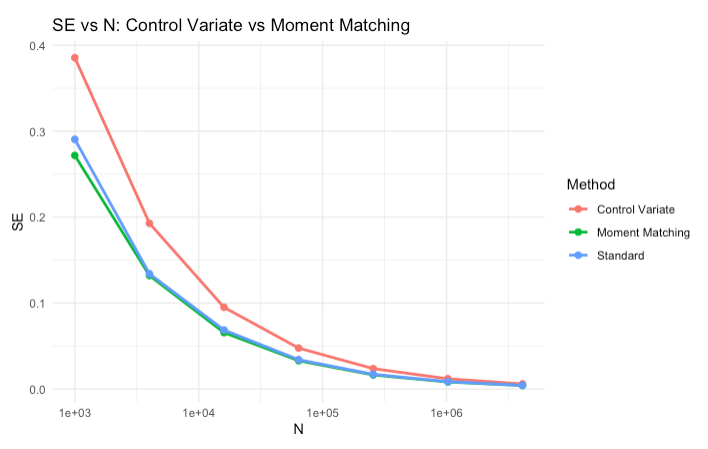
\includegraphics[width=0.9\linewidth]{se_N_comparison.png}
    \caption{Comparative plot for SE across all methods}
    \label{fig:enter-label}
\end{figure}

\begin{figure}[H]
    \centering
    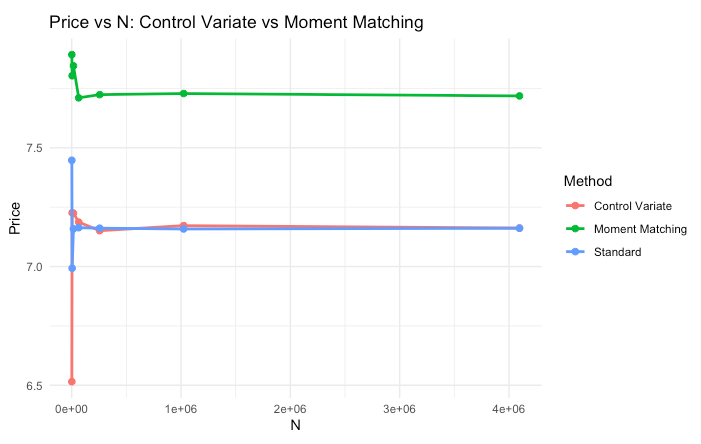
\includegraphics[width=0.9\linewidth]{price_v_N_comparison.png}
    \caption{Comparative plot for Price across all methods}
    \label{fig:enter-label}
\end{figure}
\newpage
{\color{gray}\hrule}
\begin{center}
\section{American Vanilla Put Option Pricing}
\textbf{You can add small descriptions of what the current sections describe}
\bigskip
\end{center}
{\color{gray}\hrule}
\begin{multicols}{2}
\subsection{Problem Statement}
An American vanilla put option is more flexible than a European option because it can be exercised at any point before maturity or at maturity. This flexibility adds a complexity, as the pricing depends on deciding the best time to exercise based on the movement of the price of the underlying asset.

The Longstaff Schwartz approach is a practical method for pricing American options. It works by simulating multiple possible movements for the asset price and using regression techniques to figure out the optimal exercise strategy. The payoff at any point \textit{t} is:
\[\text{Payoff} = \max(0, K - S_t)
\]
where K is the strike price, and $S_t$ is the asset price at time t.
Our goal is to study how various factors like the number of simulated paths(N), the number of time steps(M), and the regression model affect the estimated option price. We also evaluate how efficient and accurate these methods are in practical applications.
\subsection{Methodology}
To price the American put option, we use the Longstaff-Schwartz Monte Carlo (LSM) method. This approach leverages regression techniques to estimate the continuation value at each step and determine the optimal exercise strategy.
\subsubsection{Simulation of Asset Prices}
Simulate \(N\) independent paths for the underlying asset price using the geometric Brownian motion (GBM) model:
\[
dS_t = (r - q) S_t \, dt + \sigma S_t \, dW_t,
\]
where \(dW_t\) represents the Wiener process.

Discretize the GBM equation using the time step \(\Delta t = \frac{T}{M}\) and simulate the price paths at each time step:
\[
S_{t+\Delta t} = S_t e^{(r - q - \frac{\sigma^2}{2}) \Delta t + \sigma \sqrt{\Delta t} Z},
\]
where \(Z \sim N(0,1)\) is a standard normal random variable.

\subsubsection{Payoff Calculation}
At each time step, calculate the payoff if the option is exercised immediately:
\[
\text{Payoff} = \max(0, K - S_t).
\]

\subsubsection{Regression for Continuation Value}
Starting from the second-to-last time step (\(t_{M-1}\)) and moving backward:
\begin{itemize}
    \item Use regression to estimate the continuation value of the option:
    \[
    \mathbb{E}[V_{t+1} \mid S_t],
    \]
    where \(V_{t+1}\) is the option value at the next time step.
    \item Fit a polynomial of degree \(K_{\text{reg}}\) (e.g., 2 or 3) to approximate the continuation value as a function of \(S_t\).
    \item Compare the continuation value with the immediate exercise value:
    \begin{itemize}
        \item If the immediate exercise value exceeds the continuation value, exercise the option.
        \item Otherwise, continue holding the option.
    \end{itemize}
\end{itemize}

\subsubsection{Discounting to Present Value}
For each path, calculate the discounted value of the option based on the optimal exercise strategy:
\[
V = e^{-rT} \cdot \text{Payoff}.
\]
Average these discounted values across all simulated paths to estimate the option price.

\subsubsection{Parameters Studied}
The following parameters are varied to analyze their impact on pricing accuracy and convergence:
\begin{itemize}
    \item \textbf{Sample size (\(N\)):} Increasing \(N\) reduces the stochastic error and stabilizes the price.
    \item \textbf{Number of time steps (\(M\)):} Larger \(M\) reduces time discretization error, improving accuracy.
    \item \textbf{Regression order (\(K_{\text{reg}}\)):} Affects the approximation of the continuation value.
\end{itemize}

\subsubsection{Binomial Black-Scholes with Richardson Extrapolation (BBSR)}
For American options, the Binomial Black-Scholes with Richardson Extrapolation (BBSR) method improves the accuracy of pricing American options by refining the standard binomial model. It works by using smaller time steps in the calculation and then applying extrapolation to estimate the option price as if the time steps were infinitely small. This reduces errors and gives highly accurate results. BBSR is especially helpful for American options because it can effectively handle the complexity of early exercise. Comparing these accurate results with those from the Longstaff-Schwartz method helps assess how affective the Monte Carlo method is.
\subsection{Results}

\subsubsection{Convergence Analysis for American Put Options}
The results demonstrate the impact of sample size (\(N\)), time steps (\(M\)), and regression order (\(K_{\text{reg}}\)) on the accuracy and stability of the Longstaff-Schwartz Monte Carlo (LSM) method for pricing American options.

\textbf{1. Effect of Sample Size (\(N\)):}  
As the number of simulated paths \(N\) increases, the estimated option price becomes progressively more stable and convergent (Figure 7).

\begin{itemize}
    \item At small \(N\) (e.g., \(N = 1,000\)), the option prices exhibit significant dispersion and volatility due to stochastic errors.
    \item As \(N\) increases to values like \(10,000\), the dispersion reduces, and prices cluster around the true value (approximately 2.22).
\end{itemize}
This highlights the importance of sufficient sample size to average out randomness and achieve stable results.

\textbf{2. Effect of Time Steps (\(M\)):}  
Time discretization plays a crucial role in pricing accuracy (Figure 8).

\begin{itemize}
    \item When \(M\) is small (e.g., \(M < 1,000\)), time discretization errors lead to significant volatility, especially for smaller \(N\).
    \item As \(M\) increases (e.g., \(M \geq 3,000\)), the prices stabilize, reducing variability and improving accuracy.
\end{itemize}
The convergence trend becomes clear when both \(N \geq 3,000\) and \(M \geq 2,000\), where the results stabilize within a narrow range (2.2 to 2.3).

\textbf{3. Effect of Regression Order (\(K_{\text{reg}}\)):}  
The regression order in the LSM method impacts the approximation of continuation values (Figure 5).
\end{multicols}
\begin{figure}
    \centering
    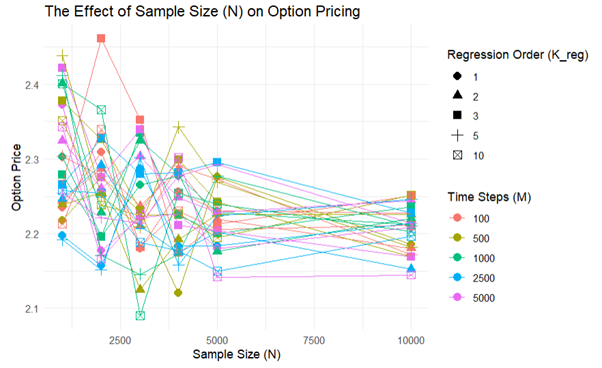
\includegraphics[width=0.9\linewidth]{Picture1.png}
    \caption{Option Price - Sample Size}
    \label{fig:enter-label}
\end{figure}
\begin{figure}
    \centering
    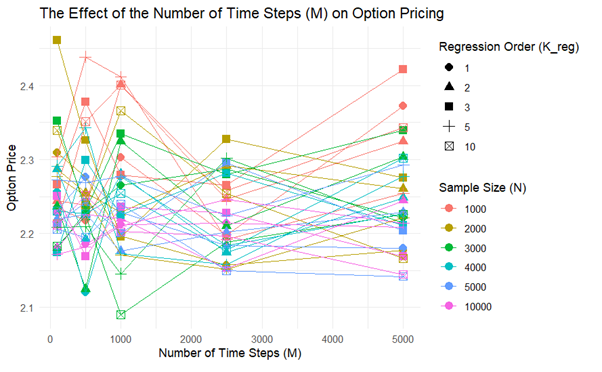
\includegraphics[width=0.9\linewidth]{Picture2.png}
    \caption{Option Price - Time Steps}
    \label{fig:enter-label}
\end{figure}

\begin{figure}[H]
    \centering
    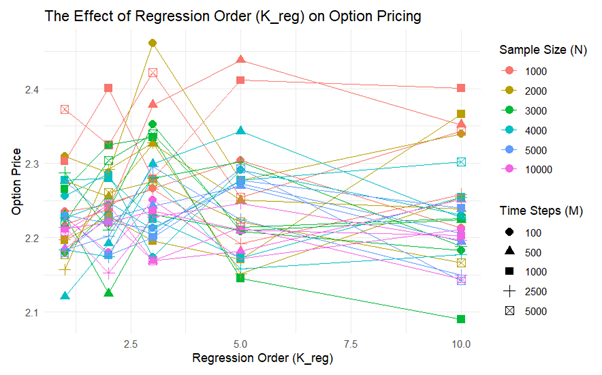
\includegraphics[width=0.9\linewidth]{Picture3.png}
    \caption{Option Price - Regression Order}
    \label{fig:enter-label}
\end{figure}
\begin{multicols}{2}
\begin{itemize}
    \item \textbf{Low Regression Orders (\(K_{\text{reg}} \leq 3\)):} These provide stable and reliable results, particularly for larger \(N\) (e.g., \(N = 5,000\)).
    \item \textbf{High Regression Orders (\(K_{\text{reg}} \geq 5\)):} These can lead to instability due to overfitting, especially when \(N\) is small or \(M\) is sparse.
\end{itemize}
For practical purposes, a regression order of \(K_{\text{reg}} = 2 \sim 3\) offers a good balance between accuracy and stability.

\subsubsection{Comparison of LSM and BBSR Methods}
The comparison between the Longstaff-Schwartz Monte Carlo (LSM) method and the Binomial Black-Scholes with Richardson Extrapolation (BBSR) method reveals the following insights(Figure 9).
\end{multicols}
\begin{table}[h!]
\centering
\caption{Comparison of LSM and BBSR Prices for Various Parameters}
\begin{tabular}{|p{1.5cm}|p{1.5cm}|p{1.5cm}|p{2.5cm}|p{2.5cm}|}
\hline
\textbf{\(N\)} & \textbf{\(M\)} & \textbf{\(K_{\text{reg}}\)} & \textbf{LSM Price} & \textbf{BBSR Price} \\ \hline
1,000  & 100  & 2 & 2.16602 & 2.215176 \\ \hline
1,000  & 100  & 3 & 2.347223 & 2.215176 \\ \hline
1,000  & 100  & 5 & 2.312833 & 2.215176 \\ \hline
1,000  & 500  & 2 & 2.156658 & 2.223767 \\ \hline
1,000  & 500  & 3 & 2.211544 & 2.223767 \\ \hline
1,000  & 500  & 5 & 2.205814 & 2.223767 \\ \hline
1,000  & 1000 & 2 & 2.209214 & 2.224865 \\ \hline
1,000  & 1000 & 3 & 2.209717 & 2.224865 \\ \hline
1,000  & 2500 & 2 & 2.25208  & 2.225478 \\ \hline
\end{tabular}
\label{tab:LSM_vs_BBSR_1}
\end{table}
\begin{multicols}{2}

\textbf{1. Stability of the BBSR Method:}  
The BBSR method produces highly stable option prices, even for small \(N\) and \(M\), with prices consistently within a narrow range (approximately 2.215 to 2.225). This highlights its superior accuracy and makes it a reliable benchmark.
\end{multicols}
\begin{table}[h!]
\centering
\caption{Comparison of LSM and BBSR Prices for Larger Sample Sizes}
\begin{tabular}{|p{1.5cm}|p{1.5cm}|p{1.5cm}|p{2.5cm}|p{2.5cm}|}
\hline
\textbf{\(N\)} & \textbf{\(M\)} & \textbf{\(K_{\text{reg}}\)} & \textbf{LSM Price} & \textbf{BBSR Price} \\ \hline
10,000 & 100  & 2 & 2.25674 & 2.215176 \\ \hline
10,000 & 100  & 3 & 2.18681 & 2.215176 \\ \hline
10,000 & 100  & 5 & 2.22371 & 2.215176 \\ \hline
10,000 & 500  & 2 & 2.20556 & 2.223767 \\ \hline
10,000 & 500  & 3 & 2.215695 & 2.223767 \\ \hline
10,000 & 500  & 5 & 2.219789 & 2.223767 \\ \hline
10,000 & 1000 & 2 & 2.224479 & 2.224865 \\ \hline
10,000 & 1000 & 3 & 2.230177 & 2.224865 \\ \hline
10,000 & 2500 & 2 & 2.263049 & 2.225478 \\ \hline
\end{tabular}
\label{tab:LSM_vs_BBSR_2}
\end{table}

\begin{multicols}{2}
\textbf{2. Convergence of the LSM Method:}  
The LSM method shows more volatility for small \(N\) (e.g., \(N = 1,000\)) and small \(M\) (e.g., \(M = 100\)). However, as \(N\) and \(M\) increase:
\begin{itemize}
    \item LSM prices converge toward the BBSR benchmark.
    \item The scatter observed at smaller \(N\) and \(M\) reduces, with results stabilizing around the true option price.
\end{itemize}
\subsection{Discussion}
The results of pricing the American put option using the Longstaff-Schwartz Monte Carlo (LSM) method and the Binomial Black-Scholes with Richardson Extrapolation (BBSR) method highlight important findings regarding accuracy, convergence, and computational efficiency.

\subsubsection{Stability and Accuracy of the BBSR Method}
The BBSR method consistently produced stable and accurate option prices, even with smaller time steps (\(M\)) and sample sizes (\(N\)). We assume this stability is caused by its ability to improve results using Richardson extrapolation, which effectively eliminates discretization errors i.e errors caused due to the discrete approximation of a continuous process. In all cases, the BBSR prices remained within a narrow range of approximately 2.215 to 2.225, making it really useful for evaluating the LSM method.

\textbf{The key advantages of the BBSR method include:}
\begin{itemize}
    \item \textbf{High Accuracy:} Prices are consistently close to the true option value.
    \item \textbf{Reduced Sensitivity:} Results are less affected by changes in \(N\) which \(M\), makes the method computationally efficient for smaller datasets.
    \item \textbf{Ease of Implementation:} The method provides reliable estimates without requiring approximations from the regression model in the LSM method.
\end{itemize}
However, the BBSR method is limited to simpler models and may not generalize as effectively for more complex derivatives which can have higher number of dependencies.

\subsubsection{Convergence and Efficiency of the LSM Method}
The Longstaff-Schwartz method showed strong performance, particularly for larger \(N\) and \(M\), while converging to the BBSR values. However, the results show that LSM is sensitive to a few key parameters:

\textbf{Sample Size (\(N\)):}  
\begin{itemize}
    \item At smaller values of \(N\) (e.g., \(N = 1,000\)), the option prices had significant volatility, reflecting the stochastic nature of Monte Carlo simulations.
    \item As \(N\) increased, the random noise reduced, and the prices stabilized close to the benchmark (e.g., \(N = 10,000\)).
\end{itemize}

\textbf{Number of Time Steps (\(M\)):}  
\begin{itemize}
    \item Time discretization errors were observed for smaller \(M\) (e.g., \(M = 100\)).
    \item Increasing \(M\) (e.g., \(M \geq 1,000\)) reduced these errors, improving the accuracy of the continuation value approximation.
\end{itemize}

\textbf{Regression Order (\(K_{\text{reg}}\)):}  
\begin{itemize}
    \item For \(K_{\text{reg}} \leq 3\), the LSM method provided stable and accurate estimates.
    \item Higher regression orders (\(K_{\text{reg}} \geq 5\)) led to overfitting, particularly for smaller \(N\), introducing unnecessary variability.
    \item A regression order of \(K_{\text{reg}} = 2\) or \(3\) strikes the best balance between accuracy and computational efficiency.
\end{itemize}

\subsubsection{Computational Performance and Tradeoffs}
The BBSR method is computationally efficient for small datasets but becomes resource-intensive as time steps increase. The LSM method, while computationally heavier due to the need for multiple regressions, offers flexibility in handling early exercise features and complex models.

\textbf{The following tradeoffs are observed:}
\begin{itemize}
    \item \textbf{Accuracy vs. Computational Cost:}  
    While the LSM method requires a larger \(N\) and \(M\) to converge, the compute time increases significantly. For practical purposes, values such as \(N = 10,000\) and \(M = 1,000\) are recommended for balancing accuracy and efficiency.
    
    \item \textbf{Regression Complexity:}  
    Higher regression orders provide diminishing returns and increase compute time without significant improvements in the accuracy.
\end{itemize}

\subsubsection*{4. Practical Recommendations}
\begin{itemize}
    \item For applications where accuracy is critical and computational resources are limited, the BBSR method should be selected due to its stability.
    \item The Longstaff-Schwartz method is well-suited for scenarios requiring flexibility in handling path-dependent options or early exercise features. 
    \item Future improvements can include combining the LSM method with variance reduction techniques such as antithetic variates or control variates to further reduce variability and compute cost.
\end{itemize}

\subsubsection{Future Directions}
\begin{itemize}
    \item \textbf{Variance Reduction:} Implement variance reduction techniques (e.g., antithetic variates, control variates, stratified sampling) to enhance the efficiency of the LSM method.
    \item \textbf{Parallelization:} Use parallel computing to accelerate Monte Carlo simulations, particularly for large sample sizes.
    \item \textbf{Comparison with Other Methods:} Compare the LSM and BBSR methods with other techniques like Finite Difference Methods (FDM) or Quasi-Monte Carlo methods to analyze their accuracy and efficiency further.
    \item \textbf{Complex Derivatives:} Extend the analysis to other path-dependent options, such as barrier options or options with stochastic volatility.
\end{itemize}

The BBSR method serves as a stable and accurate benchmark for pricing American options, while the Longstaff-Schwartz method provides flexibility at the cost of higher computational requirements. The choice of method depends on the tradeoff between computational efficiency and model complexity. By optimizing sample size, time steps, and regression parameters, the LSM method can achieve results close to the BBSR benchmark while maintaining computational feasibility.
\end{multicols}
\newpage
{\color{gray}\hrule}
\begin{center}
\section{Efforts to Reduce Computational Time}
% \textbf{Small description}
\bigskip
\end{center}
{\color{gray}\hrule}
\begin{multicols}{2}
\subsection{Summary of computational time improvements}
To efficiently conduct Monte Carlo simulations that exceed 1 million underlying asset price path simulations per valuation, we employed the C++ programming language for its superior performance capabilities over Python or R. However, as the scale of simulations further increased, the computational efficiency of the initial, unoptimized C++ implementation was proved to be inadequate. For instance, the computation time averaged 40.71 seconds to price a European put option with 10 million simulations. Such an evident decline in performance underscored the need for parallel programming techniques, specifically multithreading, to accelerate the computational process.

Upon the implementation of the multithreading technique, as detailed in the subsequent section, the average computation time was reduced to 7.86 seconds, representing an approximate fivefold improvement in time efficiency. To achieve further acceleration, GPU programming frameworks like CUDA that leverage parallel processing within the GPU could be explored.
\subsection{Methods employed to optimize code performance}
\subsubsection{Multithreading}
Multithreading is a parallel programming technique that divides the computation task into smaller independent subtasks that concurrently run on different CPU cores. This workload parallelization lowers the wall-clock time relative to single-thread execution. In the context of Monte Carlo simulations, this method enables faster computation by assigning a certain number of underlying asset price development simulations and the corresponding option contract valuation to each thread.

We first determined the number of available logical cores supported by the system to evenly distribute the number of simulations among them. Once the threads are launched, each thread executes its subset of simulations independently and computes the option price and the corresponding statistics. To prevent data inconsistency due to multiple threads attempting to modify shared resources simultaneously, we used mutex (mutual exclusion) class to ensure thread-safe updates when accessing shared data structures. Once all threads complete their tasks, the main thread combines the results from each thread to compute the overall simulation statistics.
\subsubsection{Memoization}
Memoization is a computational optimization technique that reduces redundant calculations by storing previously computed results for reuse in subsequent operations. Memoization is employed while computing the American options using the Black-Scholes binomial tree method to store underlying asset prices and the previous step's option values during backward induction.

A key property leveraged during the construction of the underlying asset price tree is the symmetry at each level. While computing the binomial underlying asset prices the upward and downward movements cancel out, ensuring $S \cdot u \cdot d = S$. This property reduces the need to compute all possible price levels at each iteration explicitly, as they can be derived from a single upward or downward step relative to the previous node.

This approach significantly reduces the time and space complexity of the algorithm from exponential to quadratic.
\end{multicols}
\newpage
{\color{gray}\hrule}
\begin{center}
\section{Conclusions}
\bigskip
\end{center}
{\color{gray}\hrule}
\vspace{0.5cm}
Our main objective with this project was to explore the application of Monte Carlo simulations for pricing various types of options—European vanilla put options, Asian call options, and American vanilla put options—under the Black-Scholes-Merton framework. Alongside understanding option payoffs and their mathematical formulas, we also tried to improve computational cost and reduce variance using advanced numerical techniques.

\begin{itemize}
    \item \textbf{Monte Carlo Simulations:}  
    Monte Carlo methods proved to be effective for estimating option prices, particularly for complex payoffs like Asian options and early-exercise option of American options. The simulations followed the expected theoretical convergence rate of \( \frac{1}{\sqrt{N}} \), with increasing sample sizes significantly reducing standard errors and tightening confidence intervals.

    \item \textbf{Variance Reduction Techniques:}  
    Advanced variance reduction methods such as \textbf{control variates}, \textbf{antithetic variates}, and \textbf{moment matching} were implemented to enhance accuracy and computational efficiency:
    \begin{itemize}
        \item \textbf{Control Variates:} Used known solutions, such as the geometric Asian call price, to reduce variance without adding bias to the results.
        \item \textbf{Antithetic Variates:} Demonstrated their usefulness for pricing European options, reducing standard errors with minimal computational cost.
        \item \textbf{Moment Matching:} Applied to the Asian call option, improved convergence by making sure the simulated moments aligned with theoretical moments.
    \end{itemize}

    \item \textbf{Longstaff-Schwartz Method and BBSR Comparison:}  
    For American put options, the Longstaff-Schwartz Monte Carlo (LSM) method was compared with the Binomial Black-Scholes with Richardson Extrapolation (BBSR) approach.
    \begin{itemize}
        \item The \textbf{BBSR method} provided highly stable and accurate results.
        \item The \textbf{LSM method}, though sensitive to parameters like sample size time steps, and regression order, converged to the BBSR values with computational effort.
    \end{itemize}

\end{itemize}

This project not only deepened our understanding of Monte Carlo simulations for option pricing but also highlighted the importance of balancing numerical techniques with computational efficiency. By integrating numerical methods with optimized coding practices, we successfully developed a framework that can be applied to solve real-world financial problems efficiently and accurately.

\newpage
{\color{gray}\hrule}
\begin{center}
\section{Appendices}
%\textbf{Small description}
\bigskip
\end{center}
{\color{gray}\hrule}
\begin{multicols}{2}
\subsection{Code Structure}
\begin{verbatim}
    exec
     |   - main // Executable
    include
     |   - AmericanOption.cpp
     |   - AmericanOption.h
     |   - AsianOption.cpp
     |   - AsianOption.h
     |   - EuropeanOption.cpp
     |   - EuropeanOption.h
     |   - MonteCarlo.h
     |   - Option.h
    lib  {external libraries}
     |   - boost/
     |   - eigen/
    src
     |   - main.cpp
\end{verbatim}
\subsection{Definitions}
\begin{itemize}
    \item \textbf{Discretization Errors:} Errors that may arise when continuous mathematical features like time are approximated using discrete steps in numerical simulations.
    \item \textbf{Continuation Value Approximation:} The continuation value in option pricing refers to the expected value of holding an option and not exercising it immediately, under a risk-neutral measure.
    \item \textbf{Regression Order:} The regression order refers to the degree of the polynomial used to approximate the continuation value of the option. A higher regression order allows for a more flexible and accurate fit of the continuation value function to the simulated asset prices. 
    \item \textbf{Geometric Brownian Motion:} A stochastic process used to model the price of the underlying asset in the Black-Scholes framework.
    \item \textbf{Volatility:} A measure of the uncertainty or variability in the price of the underlying asset.
    \item \textbf{Multithreading:} A parallel programming technique that divides computational tasks among multiple CPU cores for faster performance.
    \item \textbf{Memoization:} A computational optimization technique that caches previously calculated results for reuse to avoid redundant computations.
\end{itemize}

\subsection{Graphs}
\subsubsection{LSM \& BBSR Comparison}
The graph (Figure 4) illustrates the tradeoff between computational effort and accuracy in the Longstaff-Schwartz Monte Carlo (LSM) method. While the BBSR method produces stable and accurate results across all parameters, the LSM method converges to the correct price only when the sample size (\(N\)) and the number of time steps (\(M\)) are sufficiently large.
\end{multicols}
\begin{figure}[H]
    \centering
    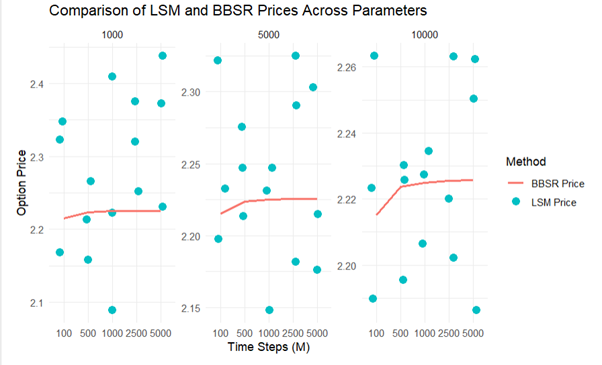
\includegraphics[width=1\linewidth]{Picture6.png}
    \caption{LSM \& BBSR Comparison}
    \label{fig:enter-label}
\end{figure}

\href{https://gitlab.engr.illinois.edu/mbhang2/ie522_final_project.git}{GitLab Code Repository}
\newpage
\bibliographystyle{plain}
\bibliography{references}
\end{document}